\chapter{Protección contra el malware}

\section{Estado actual de la protección contra malware}
Antes de la realización de esta práctica, el equipo (basado en el sistema operativo macOS) 
contaba exclusivamente con las soluciones de seguridad nativas 
de Apple, sin disponer de software antimalware de terceros instalado. Para la
realización de este apartado se instaló por recomendación de los usuarios
del foro reddit y de la ia gemini. Fue necesaria la instalación de este
software ya que el sistema operativo de Apple no cuenta con un software 
antimalware que permita realizar escaneos completos del sistema de forma 
manual, sino que se basa en mecanismos de protección integrados y 
automáticos. Estos mecanismos incluyen:
\begin{itemize}
    \item \textbf{XProtect:} Un sistema de detección de malware basado en 
    firmas que se actualiza automáticamente a través de las actualizaciones
     de macOS. XProtect escanea los archivos descargados y las aplicaciones
      en busca de malware conocido, bloqueando su ejecución si se detecta 
      una amenaza.
    \item \textbf{Gatekeeper:} Un sistema de seguridad que impide la ejecución de aplicaciones no firmadas o que no provengan de desarrolladores identificados por Apple. Gatekeeper verifica la firma digital de las aplicaciones antes de permitir su ejecución, lo que ayuda a prevenir la instalación de software malicioso.
    \item \textbf{Herramienta de eliminación de malware (MRT):} Una herramienta que se ejecuta automáticamente en segundo plano para eliminar malware conocido que pueda haber infectado el sistema. MRT se actualiza regularmente a través de las actualizaciones de macOS para garantizar la protección contra las amenazas más recientes.
    \item \textbf{Sanboxing:} macOS utiliza técnicas de sandboxing para
     aislar las aplicaciones y limitar su acceso a los recursos del 
     sistema. Esto ayuda a prevenir que el malware pueda afectar otras 
     partes del sistema o acceder a datos sensibles manteniendo dichos ficheros 
     como solo lectura.
\end{itemize}
Personalmente, considero que estas medidas de seguridad integradas en 
macOS son efectivas para proteger contra muchas amenazas comunes, 
pero no garantizan una protección completa contra todas las formas de 
malware. Sin embargo, soy reacio a la instalación de software antimalware de terceros, ya que
pueden consumir recursos e incluso soluciones populares como Avast, MCafee 
etc. han sido objeto de controversias por prácticas de recopilación de datos.
A parte, considero poco prudente dar a un software de terceros (o de fabrica) 
permiso de lectura y escritura sobre los ficheros de mi sistema, ya que en
el peor de los casos podría comprometer la seguridad personal mía (por ejemplo, 
china con sus políticas ciudadanas de ``puntos'').
Es, además, de consenso general que la mejor forma de protegerse contra el 
malware es mantener el sistema operativo y las aplicaciones actualizadas, 
evitar descargar software de fuentes no confiables y practicar buenos 
hábitos de seguridad en línea. Asimismo, el equipo que se ha analizado en
esta práctica se utiliza principalmente para tareas de desarrollo y pruebas, 
lo que reduce el riesgo de infección por malware en comparación con un 
entorno de uso general.

Por otra parte, es importante destacar que una forma efectiva de comprobar
la seguridad del equipo, sobre todo cuando se trabaja en el entorno IT
es comprobar el rendimiento del equipo, el consumo de recursos y el 
trafico de red, ya que en ocasiones existen softwares que aunque no se 
consideren malware; actuan como un malware, se instalan sin el 
consentimiento del usuario y monitorizan el uso del equipo de la misma 
forma que un malware (por ejemplo, windows copilot). 


\begin{figure}
    \centering
    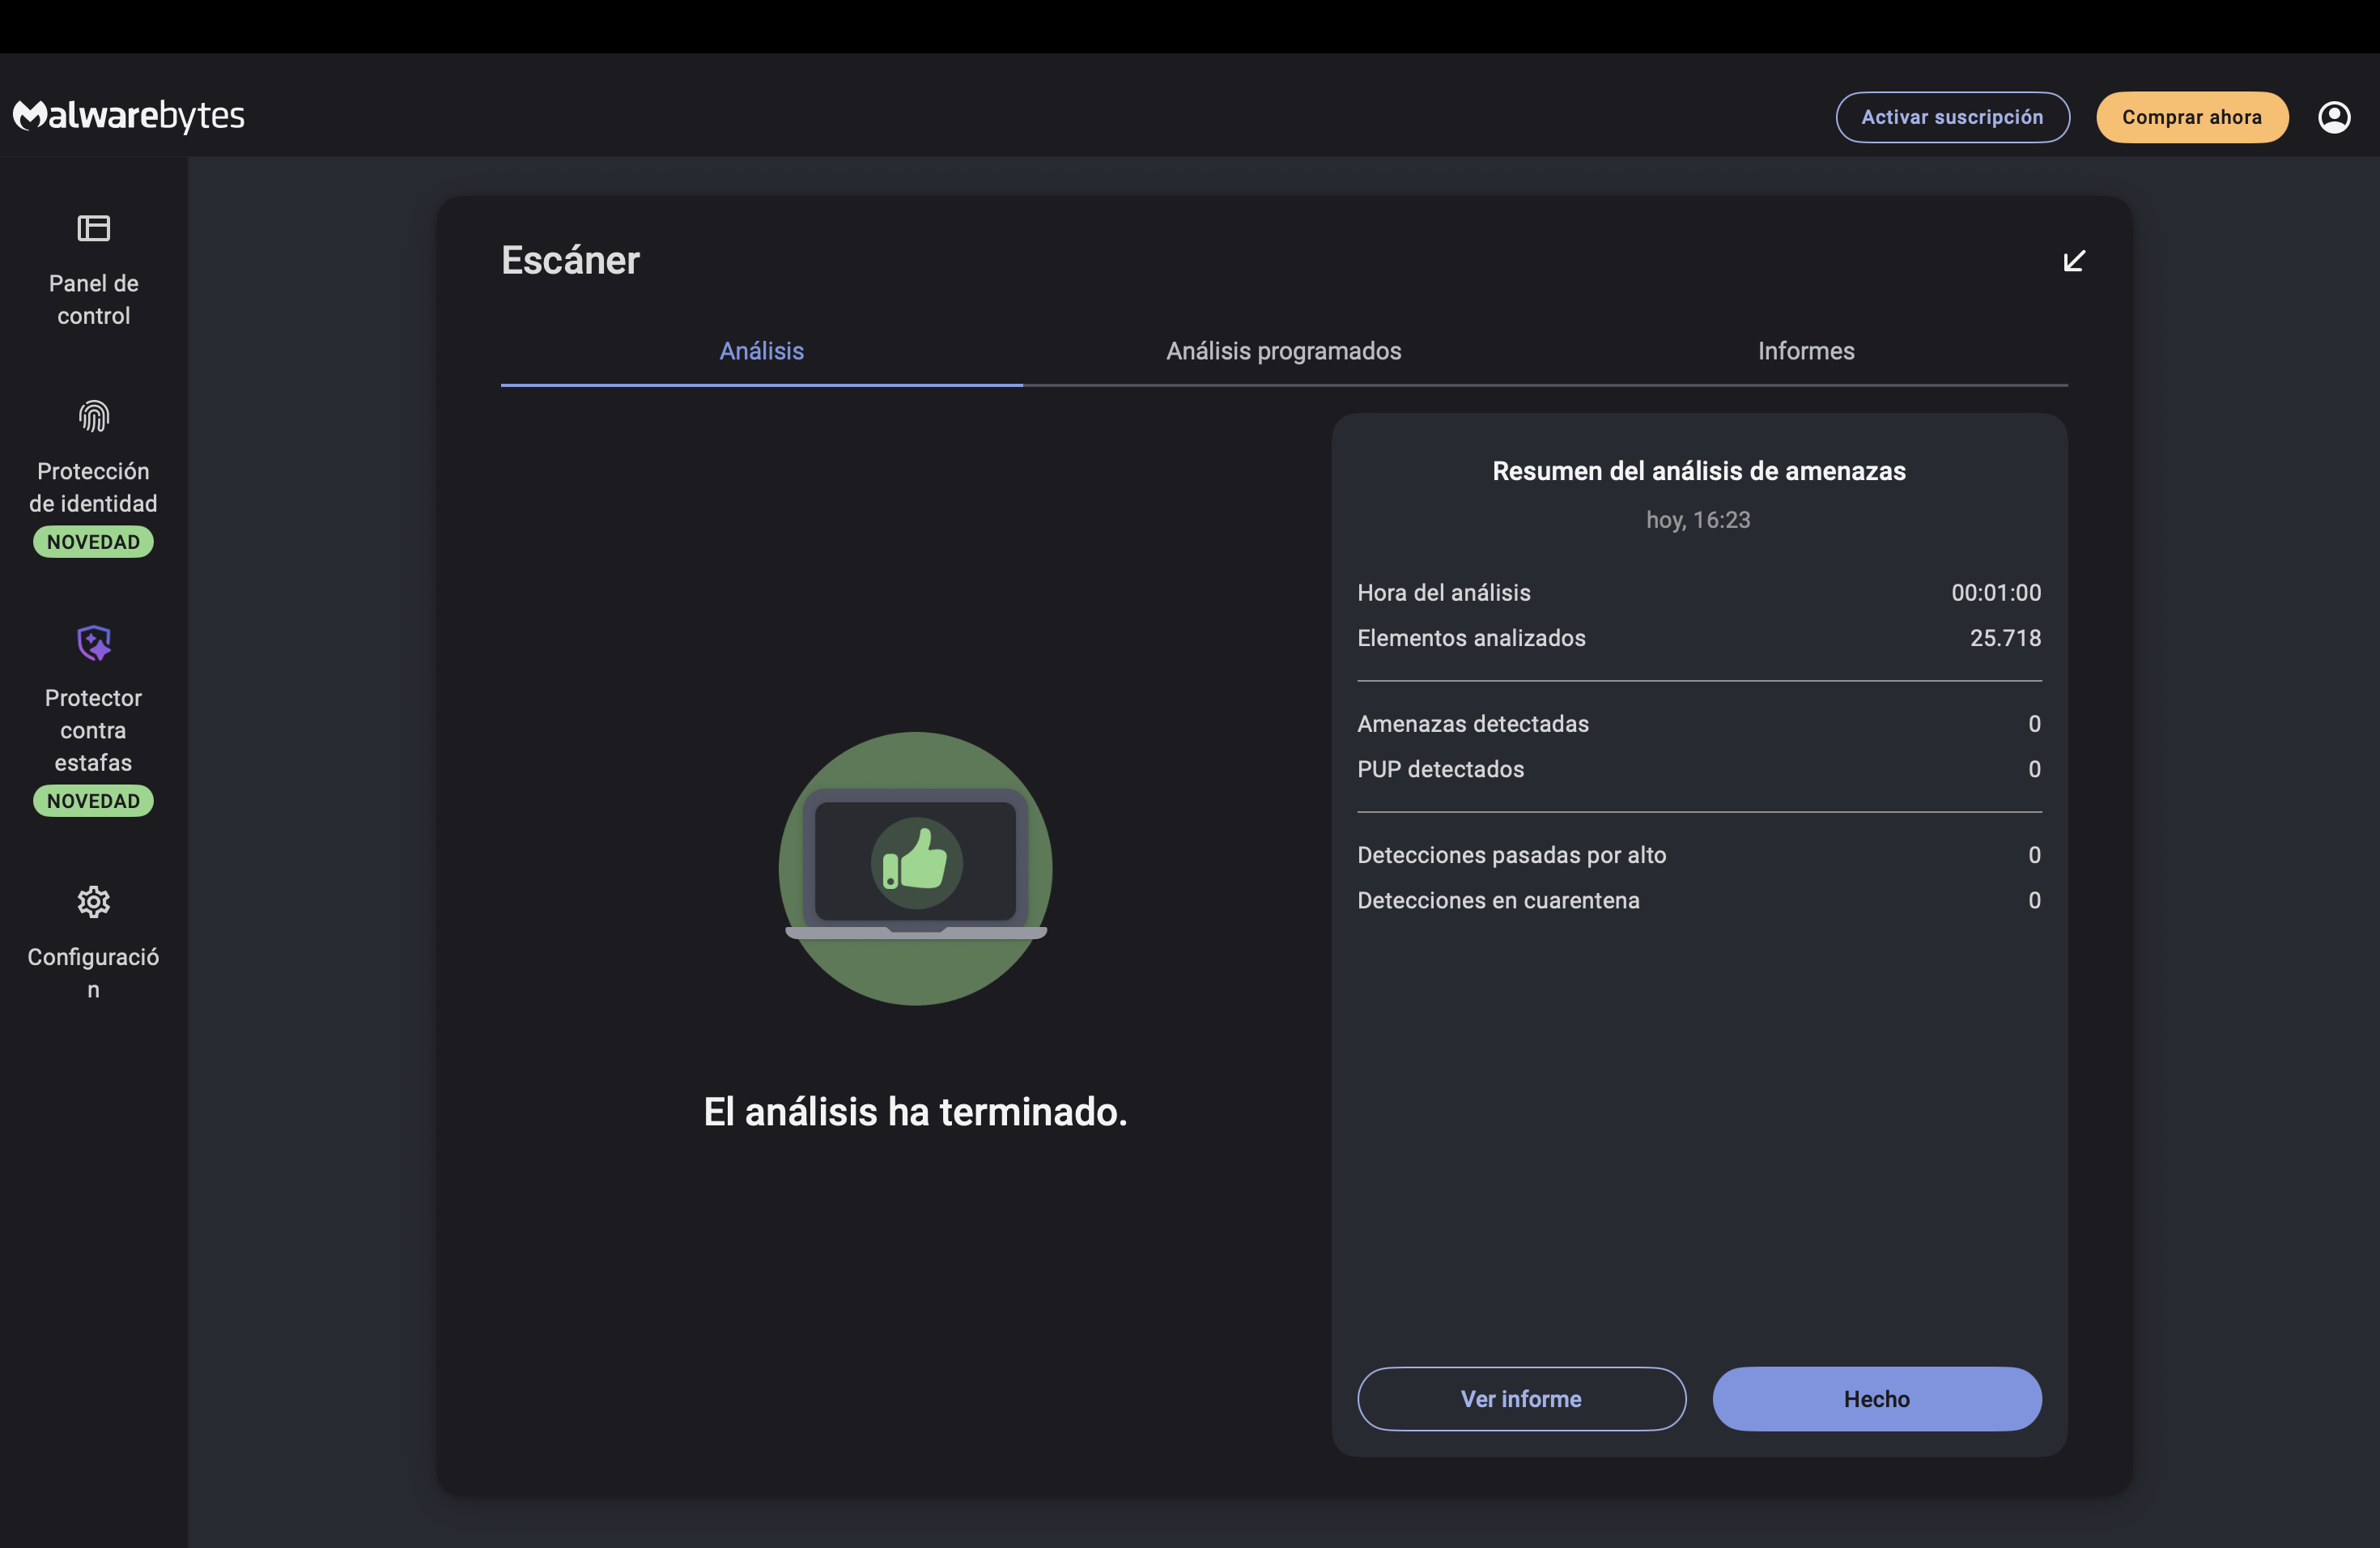
\includegraphics[width=0.8\textwidth]{Imagenes/malware1.png}
    \caption{Resultado de la comprobación malware 1.}
\end{figure}
\begin{figure}
    \centering
    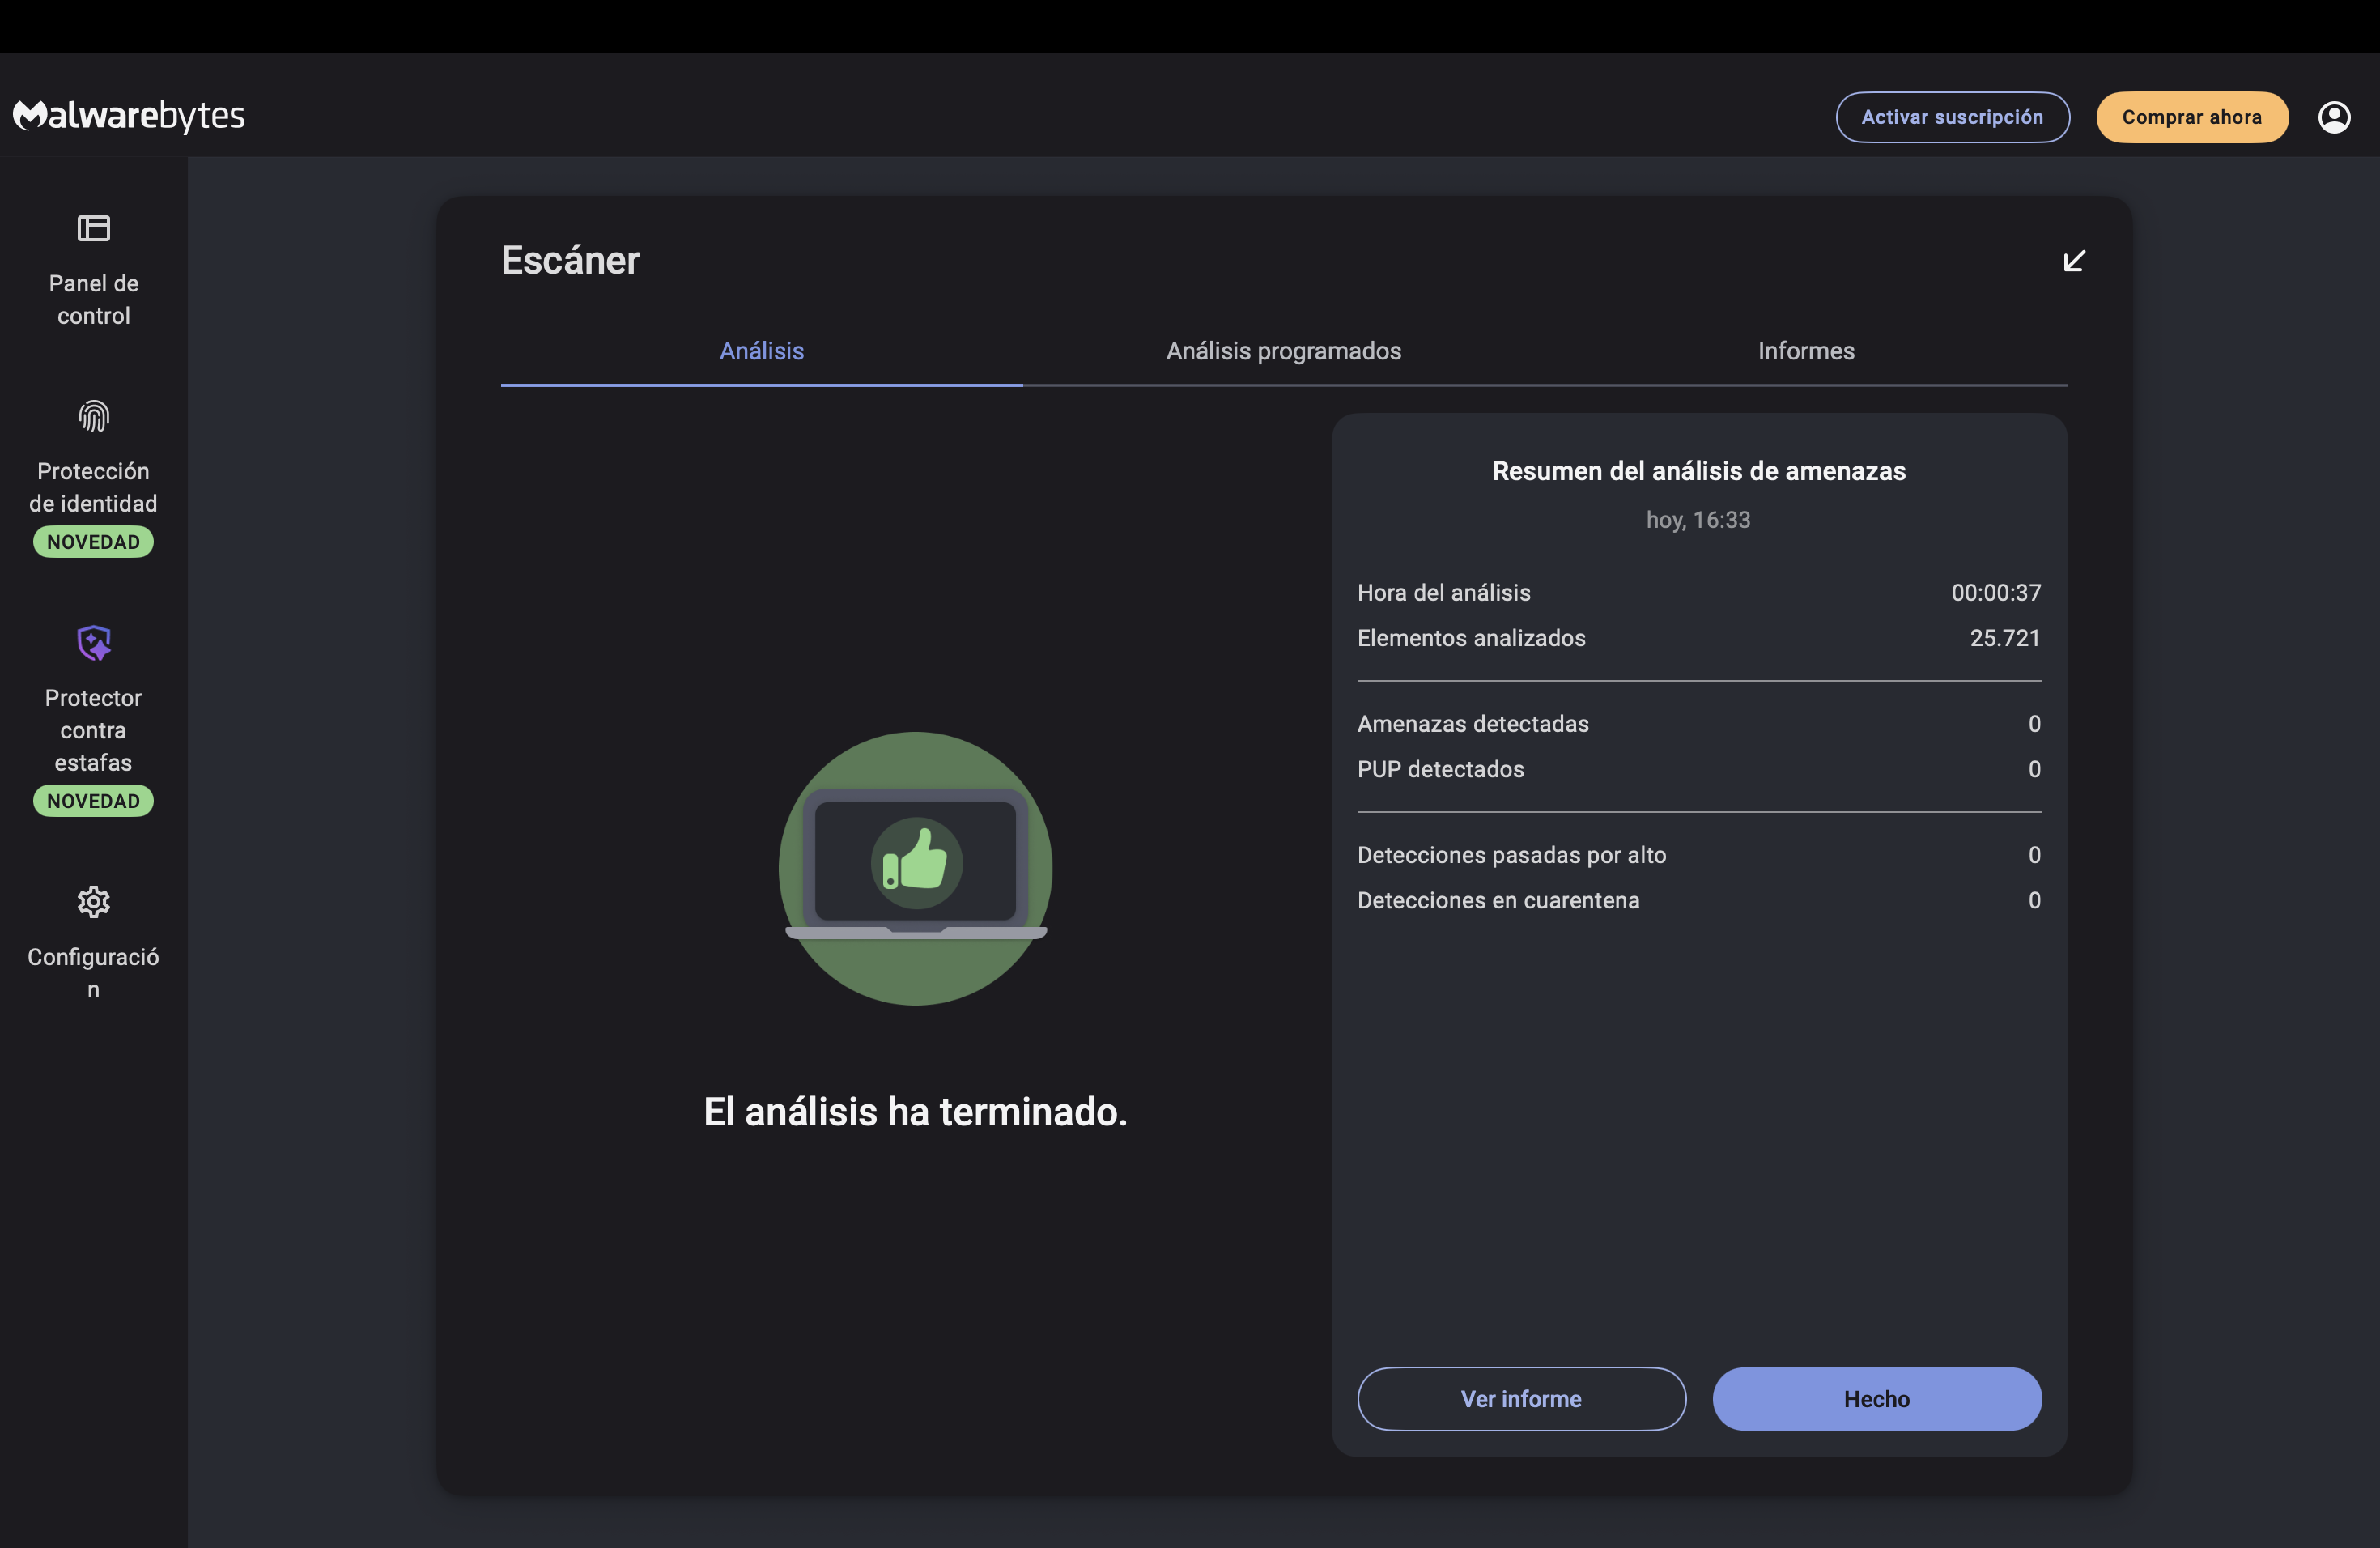
\includegraphics[width=0.8\textwidth]{Imagenes/malware2.png}
    \caption{Resultado de la comprobación malware 2.}
\end{figure}

El equipo que se ha analizado, cumple con casi todas las recomendaciones
impartidas en el manual de seguridad de la información de la unidad 1 a la 4:
Utiliza un sistema operativo actualizado, con las últimas actualizaciones de seguridad,
no tiene software de terceros instalado, no se han detectado signos de infección por malware,
utiliza en el wifi WPA2, el disco esta cifrado, se utilizan contraseñas 
seguras y autenticación multifactor, se realizan copias de seguridad 
periódicas, etc. Sin embargo, es importante destacar que la suguridad de una
red es tan fuerte como su eslabón más débil, y en este caso de estudio, el
simple hecho de que el router wifi disponga de boton wps, y que el equipo 
se conecte a este router, es un punto de vulnerabilidad importante, ya 
que el protocolo wps es vulnerable a ataques de fuerza bruta, 
lo que podría permitir a un atacante obtener acceso a la red wifi y 
comprometer la seguridad del equipo y de la red en general. 
Por lo tanto, aunque el equipo en sí mismo esté bien protegido, 
la seguridad de la red wifi a la que está conectado es un aspecto 
crítico que debe ser abordado para garantizar una protección completa 
contra el malware y otras amenazas. 